\section{Limitations of local learning}

\begin{frame}
	\frametitle{Curse of dimensionality}
	\begin{itemize}
		\item Classical non-parametric statistical learning algorithms suffer from curse of dimensionality
		\note[item]{$k$-nearest neighbors, Parzen window regression and density estimation algorithm}
	\end{itemize}
	\begin{block}{Curse of dimensionality}
		\begin{itemize}
			\item $\uparrow$ dimensionality $\Rightarrow$ $\uparrow$ volume and data becomes sparse
			\item Almost all data becomes dissimilar
			\item Statistical methods fail
		\end{itemize}
	\end{block}
	
	\begin{example}
		\begin{itemize}
			\item Density estimation in unit hypercube: $10$ bins per axis
			\item Min. $10$ samples per bin
			\item At least $n=10^d$ samples with $d$ dimension
		\end{itemize}	
	\end{example}
\end{frame}

\begin{frame}
	\frametitle{Curse of dimensionality contd.}
	\begin{itemize}
		\item Non-parametric kernel regression estimators:
		\begin{displaymath}
			\text{Expected error} = \underbrace{\frac{C_1}{n\sigma^d}}_{\text{Variance}} + \underbrace{C_2 \sigma^4}_{\text{Bias}}
		\end{displaymath}
		with $\sigma$ being the bandwidth of the kernel, $C_1$ and $C_2$ not depnding on $n$ nor on the dimension $d$ \cite{Haerdle:04}
		\item Optimal bandwidth $\sigma^{\star} \sim n^{-\frac{1}{d+4}}$
		\item Convergence rate: $n^{-\frac{4}{4+d}}$.
	\end{itemize}
	
	\begin{example}
		\begin{itemize}
			\item $d=1$: $n = n_1$ samples to obtain error $err$
			\item $d=t$: $n = n_1^{\frac{4+t}{5}}$ to obtain the same error $err$
		\end{itemize}
	\end{example}
\end{frame}

\begin{frame}
	\frametitle{Number of bases required}
	\begin{itemize}
		\item For the following: Learning models which express the learned function in terms of the training examples:
		\begin{displaymath}
			f(x) = b + \sum_{i} \alpha_i K_D(x,x_i)
		\end{displaymath}
		with $D$ being the training set
	\end{itemize}
	
	\begin{theorem}
		Let $f:\mathbb{R}\rightarrow \mathbb{R}$ computed by a Gaussian kernel machine with $k$ bases. Then $f$ has at most $2k$ zeros. \cite{Schmitt:02}
	\end{theorem}
\end{frame}

\begin{frame}
	\frametitle{Example: Learning a sinusoidal decision surface}
	\begin{columns}
		\begin{column}{6cm}
			\begin{itemize}
				\item Sinusoidal decision surface with $m$ periods
				\item Classifier has to change $2m$ times the sign
				\item Minimal number of Gaussian bases: $m$
			\end{itemize}
		\end{column}
		\begin{column}{5cm}
			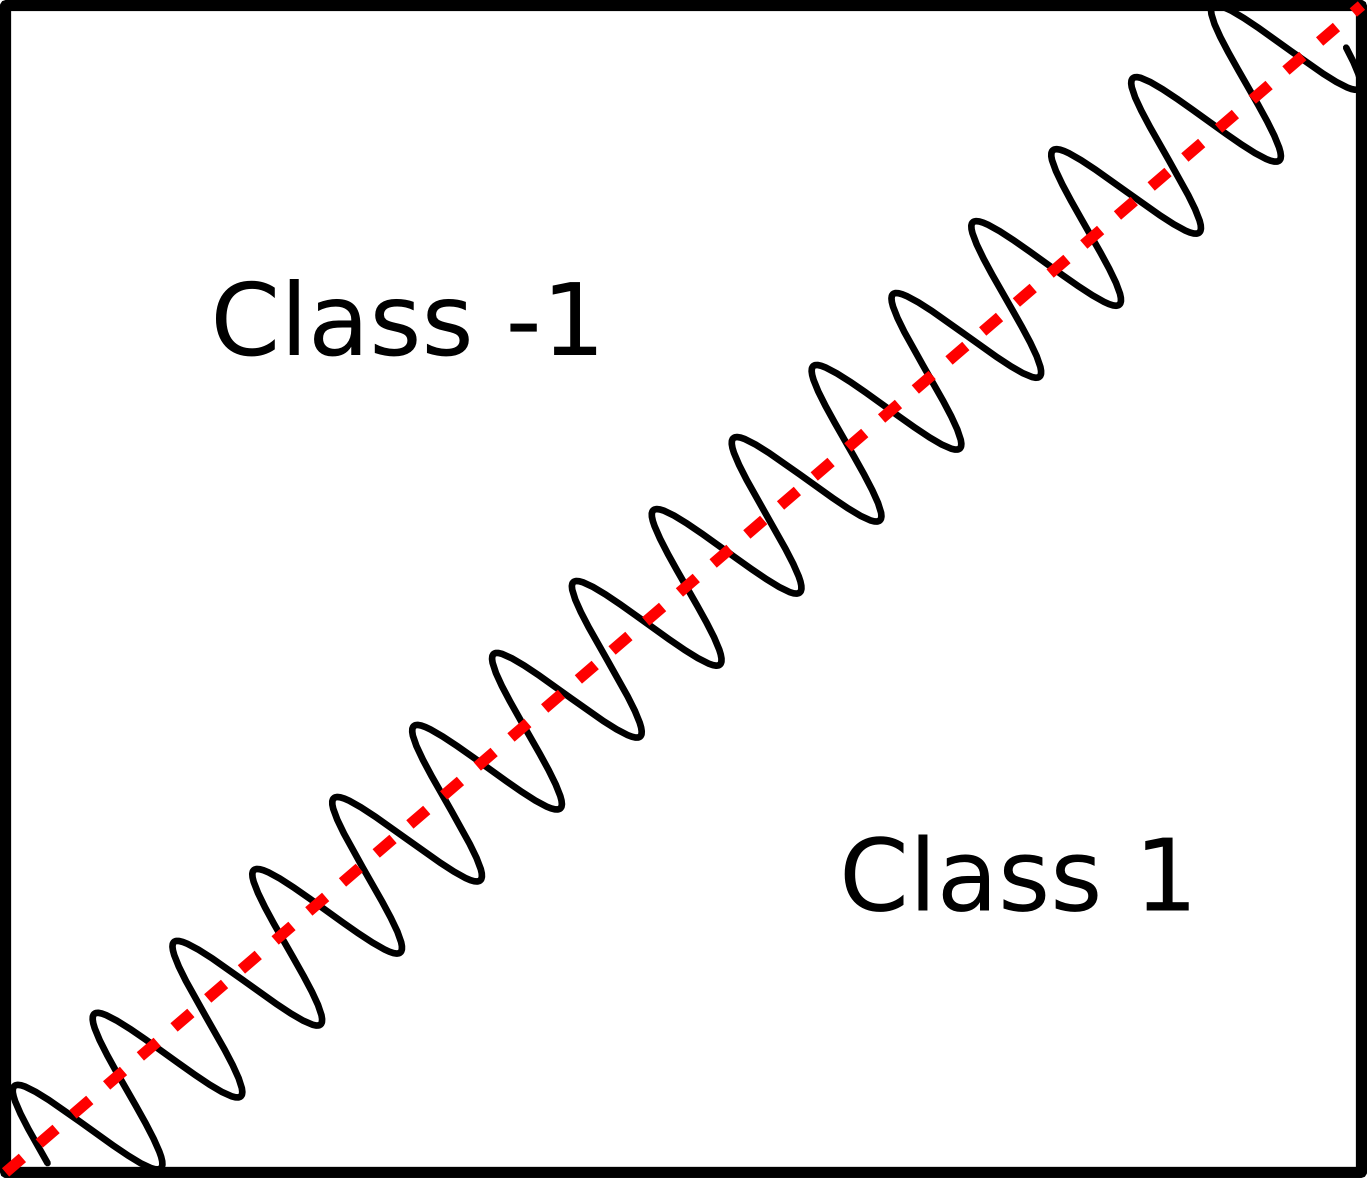
\includegraphics[width=5cm]{images/sinusoidal.png}
		\end{column}
	\end{columns}
\end{frame}

\begin{frame}
	\frametitle{Parity function}
	\begin{definition}[Parity function]
		\begin{displaymath}
			\text{parity} : (b_1,\ldots,b_d) \in \{0,1\}^d \mapsto \begin{cases}
				1 & \text{if } 2 \mid \sum_{i=1}^d b_i\\
				0 & \text{else}
			\end{cases}
		\end{displaymath}
	\end{definition}
	\begin{theorem}
		Let $f(x)=b+\sum_{i=1}^{2^d} \alpha_i K_\sigma (x_i,x)$ affine combination of Gaussians with same width $\sigma$ centered on points $x_i \in X_d$. If $f$ solves the parity problem, then there are at least $2^{d-1}$ non-zero coefficients $\alpha_i$ \cite{Bengio:06}.
	\end{theorem}
	
	\begin{itemize}
		\item Number of basis exponential in dimension $d$
	\end{itemize}
\end{frame}
